\begin{figure}[H]
\centering
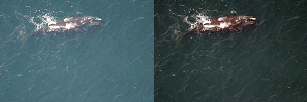
\includegraphics[width=\linewidth]{Images/preprocess1}
\caption{The first two steps in the preprocessing, left is the original image, right is the same image after normalization}
\label{fig:step1}
\end{figure}

\begin{figure}[H]
\centering
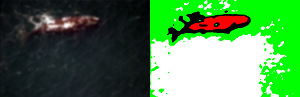
\includegraphics[width=\linewidth]{Images/preprocess2}
\caption{Left image is the right from \ref{fig:step1} smoothed, right is the left image clustered with 4 clusters}
\label{fig:step2}
\end{figure}

\begin{figure}[H]
\centering

\includegraphics[width=\linewidth]{Images/preprocess3}
\caption{Left image is the right from \ref{fig:step2} where the clusters are collapsed into two clusters, right is the original smoothed image where the water is masked out with help from the clusters}
\label{fig:step3}
\end{figure}

\begin{figure}[H]
\centering

\includegraphics[width=\linewidth]{Images/preprocess4}
\caption{Left image is second round of clustering using the image from \ref{fig:step3}, right is the resulting two clusters.}
\label{fig:step4}
\end{figure}

\begin{figure}[H]
\centering
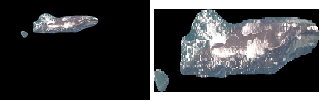
\includegraphics[width=\linewidth]{Images/preprocess5}
\caption{Left is the original image from \ref{fig:step1} with the water masked out with use of the final clusters from \ref{fig:step4}. To get from the right picture to the left a minimum bounding box is calculated, and this is used to crop the image.}
\label{fig:step5}
\end{figure}

